\section{Method}
\label{sec:method}

\subsection{Crawling Twitter}

In order to generate a significant dataset for our queries, we had to design a Python script which acts as a \emph{crawler}, going through Twitter data and storing it. That is done through the Twitter API \cite{twitterapi}. To do that, one has to sign up as a developer in twitter and obtain client credentials so that access to the API is granted to the app. The first step of the crawler script is to use these credentials so as to obtain an access token.

With access granted, our application is able to execute HTTP requests by means of the Requests library for python \cite{pyreq}. There are many possible requests offered by the Twitter API but we only used one such request, which queries the newest 100 tweets containing at least one of the hashtags given as input. It has the form: \emph{https://api.twitter.com/1.1/search/tweets.json?q=has\newline htags\&count=100\&result\_type="recent"\&lang="en"}, where "hashtags" is a string containing all the hashtags we decided were relevant for our USA elections context.

So the basic working of the script consists of an infinite loop where this request is made and the returned \emph{json} is parsed and interpreted by a set of functions which add \emph{Tweets}, \emph{Users}, \emph{Hashtags} and \emph{Words} to our database in a recursive way (i.e. if one tweet retweets a tweet that mentions a user, all this data is going to be properly processed and stored). Also, proper term extraction and stemming is done, before storing \emph{Words}.

\subsection{The Neo4j database}

Neo4j is a graph database that removes the need to explicitly define a schema
for the relationships between entities. It has efficient techniques for storing
graphs, making it suitable for storing large amounts of data with many
relationships. Neo4j allow us to represent the full structure of the Twitter
database as a graph, where each different entity is a \emph{node} and the
relationship between the nodes an \emph{edge}. Figure \ref{fig:schema} details
the nodes and the edges of our recommender engine.


% In order to store all the information fetched from Twitter, a suitable database
% had to be chosen beforehand. We wanted a solution where the relationship between
% the different entities could be easily seen and queried, and that could
% effortlessly store the large amount of data that we planned to fetch. Our
% approach utilizes a \emph{graph database} as a solution to our storing problem,
% more specifically a software called \emph{Neo4j}\cite{neo4j}. This software
% allow us to represent the full structure of the Twitter database as a graph,
% where each different entity is a \emph{node} and the relationship between the
% nodes an \emph{edge}. Figure \ref{fig:schema} details the nodes and the edges of
% our recommender engine.

The base node of the graph is the \emph{Tweet}, which is a free-text short
message sent through Twitter. Every tweet is posted by a \emph{User}, which is
represented by the \emph{post} relationship. A tweet may \emph{mention} another
user with the \emph{@} special character, and it may also \emph{tag} a topic
with \emph{\#}, represented by the node \emph{Hash}. To this basic schema
derived directly from Twitter, we added the node \emph{Word} which are all the
parsed words in the free text of the Tweet. This node is linked to the rest of
the graph through the \emph{contains} and \emph{discusses} relationships, with a
property specifying the amount of times this relationship happens for every
tweet and user. This new entity allows us to easily represent the user as a
\emph{bag-of-words} document of every word that the user discusses in all of the
user's tweets, thus allowing us to map the recommendation problem to the
standard techniques used on information retrieval.

\begin{figure}[t]
\centering
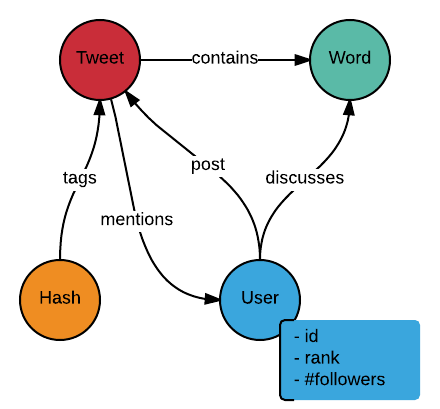
\includegraphics[width=3.0in,natwidth=440,natheight=409]{images/Schema.png}
\caption{Graph schema used for the Twitter data.}
\label{fig:schema}
\end{figure}

\subsection{Tweet text processing}

The topics of the tweets are extracted by parsing their freetext and
finding nouns and adjectives. That was an empiric decision. This is done 
using string processing alongside the Natural Language Toolkit (NLTK) 
\cite{bird2006nltk} which provides interfaces in Python for classification, 
tokenization and stemming.

\subsubsection{Cleaning tweets}

A tweet can contain hyperlinks, hashtags, mentions and other symbols. These are
removed in order to properly parse the text of the tweet. Specifically, words
starting with \verb|#, @, &, http| are ignored. A few other words that
commonly occur in a tweet were also ignored as they would not contribute to the
cause. These are \textit{don't, i'll, retweet} and \textit{rt}.

\subsubsection{Extracting topics}

First, letters are lowercased and the text is tokenized, then words shorter than
three characters are removed, after which ignored symbols are removed. Finally,
we use NLTK to Part of Speech-tag \cite{pos} each term so that we can pick only
\texttt{NN}s (nouns) and \texttt{JJ}s (adjectives) and stem these terms, which are
returned as a list.

% \subsection{Parsing tweets and extracting topics}

% The goal of the project is to recommend users given topics. In order to
% recommend a user, the user needs to be associated with the topics the user talks
% about. Therefore the users tweets are parsed and the topics of the tweets are
% extracted.  The topics are extracted by parsing the freetext of the tweets and
% extracting the nouns and adjectives.  The choice of extracting nouns and
% adjectives was an empiric decision made by the group.

% Extracting topics from tweets is done using the Natural Language Toolkit (NLTK)
% \cite{bird2006nltk} which provides interfaces in Python for things like
% classification, tokenization and stemming.

% \subsubsection{Cleaning tweets}

% A tweet can contain hyperlinks, hashtags, mentions and other symbols. These are
% removed in order to properly parse the text of the tweet. Specifically, words
% starting with \textit{\#, @, \& or http} are ignored. A few other words that
% commonly occur in a tweet were also ignored as they would not contribute to the
% cause. These are \textit{don't, i'll, retweet and rt}.

% \subsubsection{Extracting nouns}

% The nouns (topics) are extracted by performing the following actions, provided
% by NLTK:

% \begin{enumerate}
%     \item Lowercase all letters and tokenize the text into separate tokens
%     \item Remove words that are shorter than three characters (This was also a
%           decision made by the group)
%     \item For each word, remove ignored symbols and words starting with a
% 	    ignored symbol
%     \item Part of Speech-tag \cite{pos} the words
%     \item Pick the words that are tagged as \texttt{NN} (noun) or \texttt{JJ}
%         (adjective)
%     \item Stem the words and return the result which is a list of words
% \end{enumerate}

\subsection{PageRank}

One of the most well-known ranking and scoring measures is called PageRank
\cite{pr}. Made famous by Google in late 90's, its main idea is to use the
auxiliary information, mainly the \emph{link structure}, present in the World
Wide Web as an \emph{authority measure} of the web pages contained within.
Representing the web as a graph were each node is a web page and the edges the
links between a page and another, it is intuitive to see that nodes with higher
number of \emph{inlinks} (that is, the number of links arriving into a node) are
of higher importance than the ones with no inlinks at all, just like a
scientific article which is cited by several different sources, for example.

% One of the core mechanics of the algorithm is the propagation of ranking through
% links. That is, for every outlink of a web page in the graph, its ranking is
% distributed evenly among all of them. That covers both the cases when a web page
% has several different low-ranked inlinks or when it has few high-ranked ones,
% they may have similar ranks since it is not the count that matters.

% The PageRank algorithm outputs a probability, that is, the chance that an
% imaginary user will arrive at that web page, starting at any random node. The
% user interactions with web pages can be seen as a set of \emph{random walks}
% where each user follows a link until they are done surfing or they are
% \emph{bored} of following links and jump to another random web page instead.
% This bored state, which is also a probability  and normally taken as $15\%$, is
% important as to also give a score to web pages which have no inlinks at all,
% for example web pages just recently created.

\subsubsection{PageRank in the Twitter graph}

\begin{figure}[H]
\centering
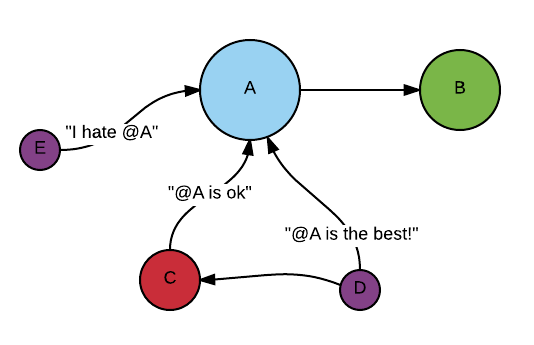
\includegraphics[width=3.5in,natwidth=534,natheight=345]{images/PageRank.png}
\caption{PageRank applied to the Twitter database. Every user is a node, while every mention in tweets is an edge. The size of the node is its relative rank among others.}
\label{fig:pagerank}
\end{figure}



Although the original PageRank algorithm was modeled with focus on the World
Wide Web, its method could be applied to any problem which can be modelled as a
graph. Specifically for Twitter, one could see each \emph{user} of the platform
as a node and every \emph{mention} in the tweets of a user to another as a link.
In the same way that web pages with high number of inlinks have a higher rank,
users that are mentioned frequently will be considered more relevant for our
recommendation engine, this process can be more clearly seen in Figure
\ref{fig:pagerank}. Note that we actually do not analyse the content of the
tweet, so tweets with positive or negative sentiment will have the same
importance for ranking, one could think of it being a "any publicity is good
publicity" kind of model.

% In our case, the probability of following a user (outlink) is proportional to
% the number of followers the corresponding user has.
The original PageRank algorithm considered following an outlink with equal
probability among all the possible links. That is reasonable with the
unstructured meta information available in the Web today, but is intuitive to
reason that, with more information about these users, different probabilities
could be applied to each one of them, depending on the task that we have at
hand. For a user recommender engine, our approach used the \emph{number of
followers} as a good measure of importance. That is, users with high number of
followers will be jumped to with higher probability in the random walk, so their
score will be naturally higher. Our engine implemented both methods for
evaluation, and the results are reported in the Experiments section.

\subsubsection{PageRank Monte Carlo}

The standard implementation of the PageRank computation is done via a method called power iteration. This method, although popular and still used today
by Google, has its drawbacks mainly regarding the speed of convergence, several
passes may be needed until the desired precision is obtained. In our approach we
explored a relatively new method, which utilize \emph{Monte Carlo algorithms} as proposed by Avrachenkov et al.
\cite{prmc} to
estimate the score of the nodes of the graph.

Of the several different algorithms proposed, our engine implements the
\emph{Monte Carlo complete path}, which is detailed in the Algorithm
\ref{alg:prmc}. For every user in the Twitter database, we start a random walk
beginning in that user and ending when the user is bored of following mentions.
We keep track of the total steps of all random walks and how many times each
user was visited. A new user is selected to be followed in the walk from all the
users the user mentions, which can be done by applying equal probabilities to
each one of them or with increased chance for higher number of followers. If a
user does not mention anyone, we consider it a \emph{sink} and jump to any other
user in the database with the same method. After every user has been at the
beginning of the random walk for a set number of walks, we calculate the user
rank by dividing the number of times each user was visited over all random walks
with the total steps taken.

\begin{algorithm}[H]
\caption{PageRank Monte Carlo, complete path}\label{alg:prmc}
\begin{algorithmic}
\Procedure{PageRank}{}
\ForAll{walks}
\ForAll{user in users}
	\State $\textit{username} \gets \textit{user['username']}$
    \State $\textit{bored} \gets \textit{False}$
    \While{$\neg bored$}
		\State $\textit{totalSteps} \gets $\textit{totalSteps} + 1
        \State $\textit{userSteps['username']} \gets \textit{userSteps['username']} + 1$
        \State $\textit{mentions} \gets \textit{getUserMentions(username)}$
     	\If{$mentions \in \emptyset$ }
                \State $\textit{username} \gets \textit{getRandomUser(users)}$
        \Else
     		\State $\textit{username} \gets \textit{getRandomUser(mentions)}$
        \EndIf
        \State $\textit{bored} \gets \textit{isUserBored()}$
    \EndWhile
\EndFor
\EndFor

\ForAll{user in users}
	\State $\textit{username} \gets \textit{user['username']}$
	\State $\textit{ranks['username']} \gets userSteps['username'] \div totalSteps $
\EndFor

\State \Return {$ranks$}

\EndProcedure
\end{algorithmic}
\end{algorithm}


\subsection{TF-IDF}

% Ranked user retrieval can be implemented by only using the aforementioned
% \emph{PageRank} algorithm but by doing so, any query would return the same top
% listed users. While that might be interesting in some applications, that is not
% the case in our context. The words in the query should also be used to filter
% and rank the retrieved users.

In order to also consider terms in the search algorithm, \emph{TF-IDF} was used, 
which is a well known solution to the problem of matching (in a ranked
way) documents modelled as \emph{bags-of-words}. Each document (including the
input query) is represented by a vector of scores, each of which related to one
of the possible terms in our dataset. The scores are calculated as follows:
${tf}_{w, d} * log_{10}(\frac{N}{{df}_{w}})$ where ${tf}_{w, d}$ is the number
of times term $w$ appears in document $d$, $N$ is the total number of documents
and ${df}_{w}$ is the number of documents term $w$ appears in. Then,
\emph{cosine-similarity} is used to compute how close the query is to each of
the documents. A link between a \emph{User} node and a \emph{Word} node maps
directly to a ${tf}_{w,d}$ score. The final procedure can be seen in Algorithm \ref{alg:tfidf}.

% In our implementation, \emph{User} nodes are documents containing each of the
% \emph{Word} nodes they are linked to. This link contains the number of times
% this \emph{Word} has been discussed by this \emph{User}, that is, a ${tf}_{w,
% d}$ score. The final procedure can be seen in Algorithm \ref{alg:tfidf}.

\begin{algorithm}[H]
\caption{TF-IDF in a Graph Database}\label{alg:tfidf}
\begin{algorithmic}
\Procedure{TF-IDF}{}
    \State $\textit{scores} \gets \emptyset$
    \State $\textit{sizes} \gets \emptyset$
    \For{token $\in$ query}
        \State $\textit{users} \gets \textit{query(users that discuss 'token')}$
        \State $\textit{df} \gets \textit{length(users)}$
        \State $\textit{count} \gets \textit{\# of occurences of 'token' in 'query'}$
        \State $\textit{wtq} \gets \textit{$count * log_{10}(\frac{length(documents)}{df})^2$}$
        \For{user $\in$ users}
        \State $\textit{tf} \gets \textit{query(\# of times 'user' discusses 'token')}$
          \State $\textit{scores[user]} \gets \textit{scores[user]} + wtq*tf$
          \State $\textit{sizes[user]} \gets \textit{query(\# of words discussed by 'user')}$
        \EndFor
    \EndFor
    \For{user $\in$ scores}
        \State $\textit{scores[user]} \gets \textit{$\frac{scores[user]}{sizes[user]}$}$
    \EndFor
    \State \Return {$sort(scores)$}
\EndProcedure
\end{algorithmic}
\end{algorithm}


\subsection{Final Score}

After retrieving the sets of \emph{PageRank} and \emph{TF-IDF} scores for all users that discuss any query term, we decided to first normalize them to zero-average and unitary variance so that they can be mixed together by means of a parameter $\alpha$. Then, the final score, for each user $u$, is: $s_{u} = \alpha * \bar{s_{p_{u}}} + (1 - \alpha) * \bar{s_{t_{u}}}$.

\subsection{Word2vec - Generating Synonyms}
Word embeddings, also referred to as distributed representations of words, is a method for generating representation of words which capture their meaning and relationships to other words. This is achieved by having each word represented by a real vector, and therefore maps each word into a multi-dimensional continuous space. In accordance to the distributional hypothesis, words which are used in similar contexts, and therefore have similar vector representations, should be mapped close to each other in the vector space. One of the most basic and widely used models is the Continuous Bag of Word (CBOW) model as described in \cite{wordRep}, which takes a context of words as input and computes the most likely target word in that context. The context words are encoded as 1-of-V vectors, where V is the size of the vocabulary, and these vectors are then averaged into one final context vector to be multiplied by the trained weight matrix of the network \cite{wordRep}.

The model used in this paper is trained using the word2vec toolkit by Google Inc \cite{word2vec}. The dataset used is the text8 file, a 97 567 kB file available from \cite{dataset}. For the training, the CBOW model was run with a word vector size of 200. The window was set to 8, negative sampling was set to 25 and 20 thread were run. Sample was set to 1e-4, binary to 1 and iterations to 15. To extract the synonyms from the trained model, the cosine and the vocab methods were called on the loaded model. The input words and the output synonyms were also cleaned in the same way as the tweets in order to gain more consistency in relation to the database.
